\documentclass{beamer}

% Theme
\usetheme{CambridgeUS}  % you can try: Warsaw, CambridgeUS, Berlin, etc.

% Packages
\usepackage[utf8]{inputenc}
\usepackage[T1]{fontenc}
\usepackage[slovene, english]{babel} % adjust if only Slovene

% Title info
\title[Ski jump predictions]{Predicting Ski Jumps using State-Space Model}
%\subtitle{Optional Subtitle}
\author{Živa Hegler and Neca Camlek}
\institute{JSI}
\date{\today}

% Change itemize bullets to red triangles
\setbeamertemplate{itemize item}{\color{darkred}\small$\blacktriangleright$}
\setbeamertemplate{itemize subitem}{\color{darkred}\scriptsize$\blacktriangleright$}
\setbeamertemplate{itemize subsubitem}{\color{darkred}\tiny$\blacktriangleright$}

%\setbeamertemplate{section in toc}{\color{black}$\bullet$~\inserttocsection}
%\setbeamertemplate{subsection in toc}{\hspace{1.2em}\color{black}$\bullet$~\inserttocsubsection}
%\setbeamertemplate{subsubsection in toc}{\hspace{2.4em}\color{black}$\bullet$~\inserttocsubsubsection}

%\setbeamertemplate{section in toc}{\color{darkred}\large\textbullet~\inserttocsection\par}
%\setbeamertemplate{subsection in toc}{\hspace{1.5em}\color{darkred}\normalsize\textbullet~\inserttocsubsection\par}
%\setbeamertemplate{subsubsection in toc}{\hspace{3em}\color{darkred}\small\textbullet~\inserttocsubsubsection\par}

\usepackage{xcolor}
\definecolor{darkred}{rgb}{0.8,0,0}

\setbeamertemplate{section in toc}{%
  \leavevmode\color{darkred}\large\textbullet\ \inserttocsection\par}
\setbeamertemplate{subsection in toc}{%
  \hspace*{1.5em}\color{darkred}\normalsize\textbullet\ \inserttocsubsection\par}
\setbeamertemplate{subsubsection in toc}{%
  \hspace*{3em}\color{darkred}\small\textbullet\ \inserttocsubsubsection\par}



\begin{document}

% Title frame
\begin{frame}
  \titlepage
\end{frame}

% Table of contents
\begin{frame}{Outline}
  \tableofcontents
\end{frame}

% Section 1
\section{Introduction}

\begin{frame}{Motivation}
  \begin{itemize}
    \item Planning of ski jump enlargement and anticipating risky conditions
    \item Goal: Predict ski jumps based on external factors
    \item Contributions
  \end{itemize}
\end{frame}

\section{Modeling Framework and Dataset}

\subsection{State-space models and Least squares method}

\begin{frame}
  \begin{itemize}
    \item State-space models (SSM)
    \item Least squares method (LS)
  \end{itemize}
\end{frame}

\subsection{Data processing}

\begin{frame}{Data Description}
  \begin{itemize}
    \item Source of data
    \item Key variables
    \item Data preprocessing steps
  \end{itemize}
\end{frame}

\begin{frame}{Images in beamer}
  %Observe Figure \ref{fig:question}: it is the
  first figure I have inserted in beamer.
  \begin{figure}
  \centering
      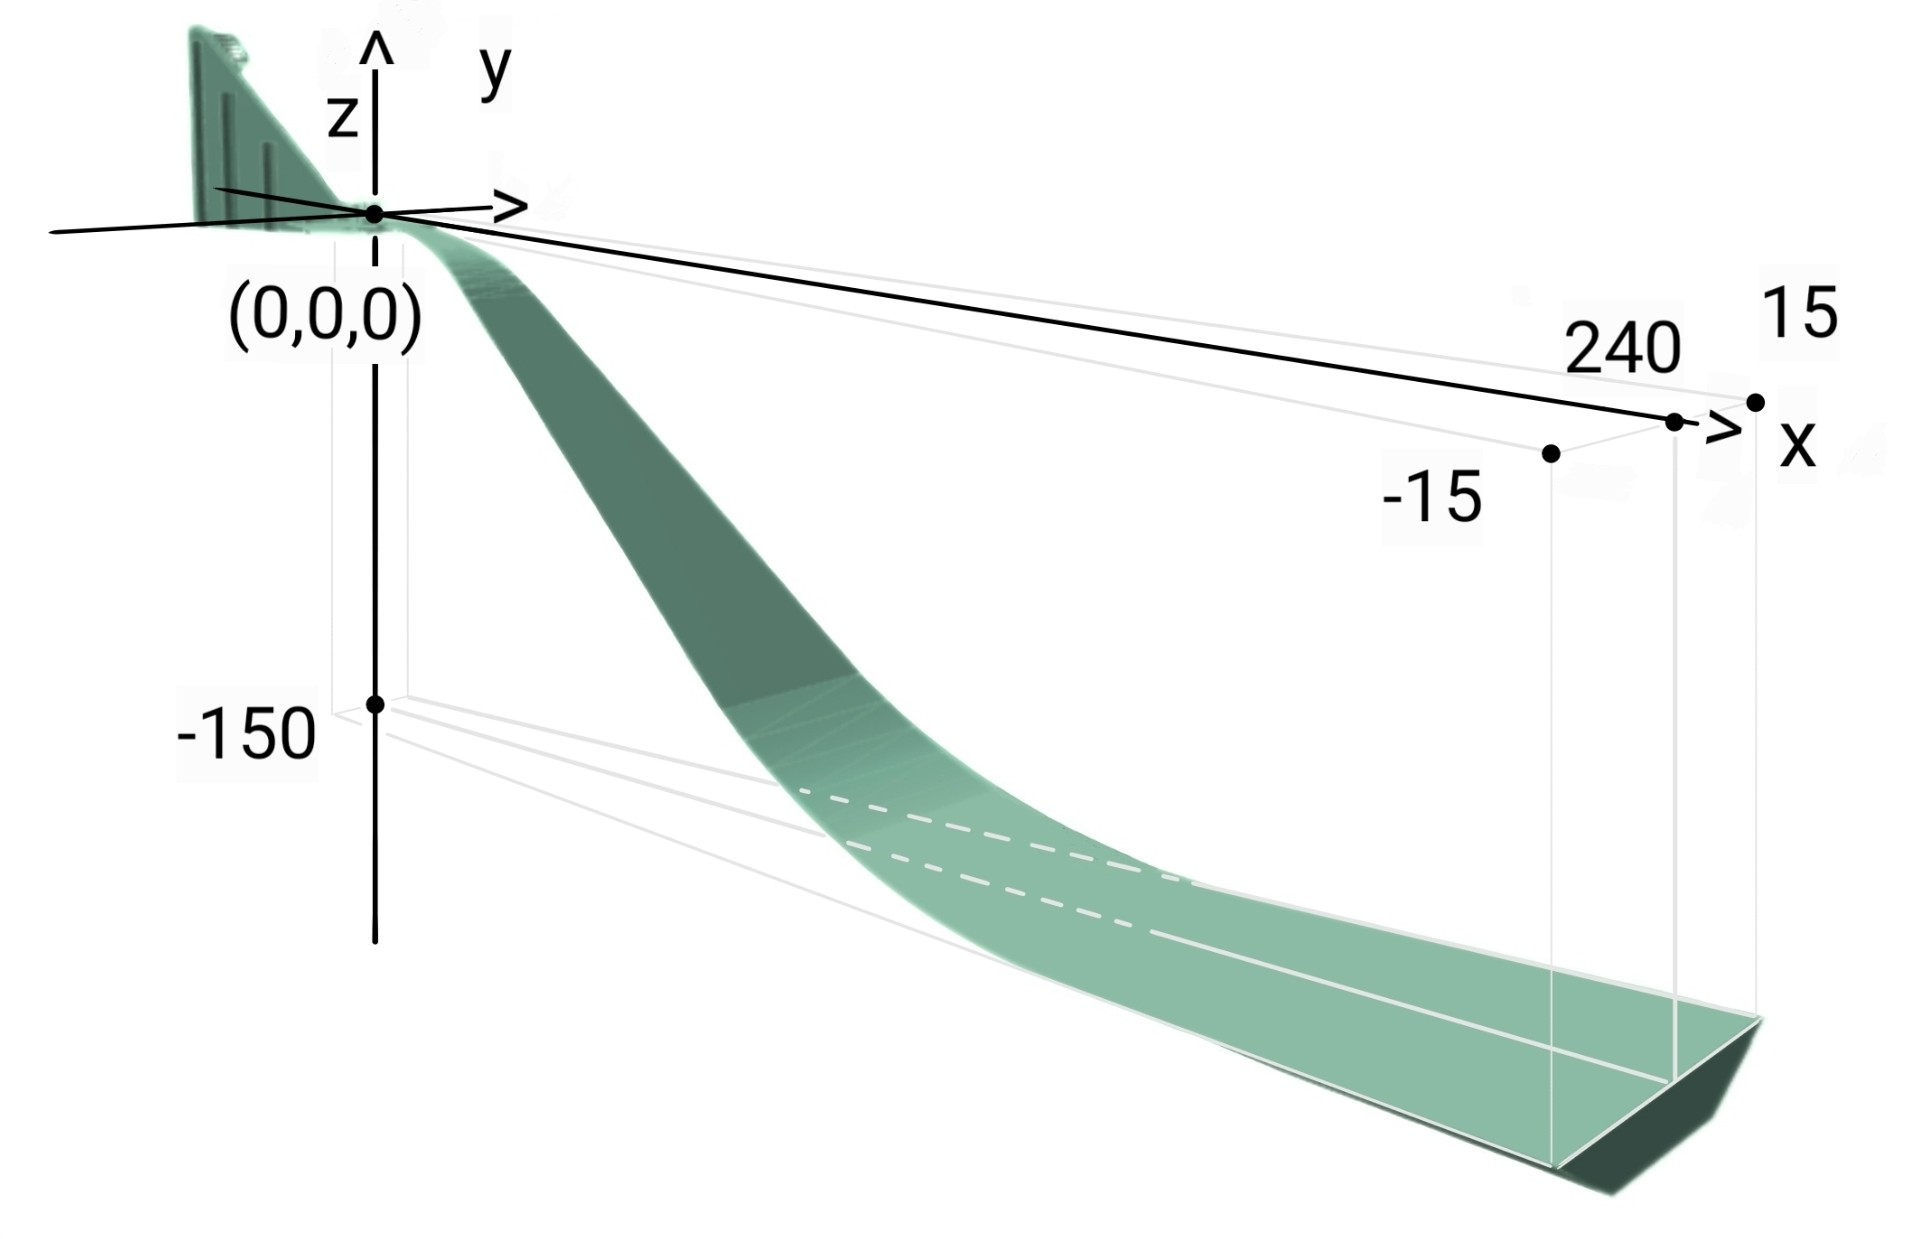
\includegraphics[width=0.5\linewidth]{planica.jpg}
      \caption{My first figure in beamer.}
      %\label{fig:question}
  \end{figure}
\end{frame}

\begin{frame}{Images in beamer}
  %Observe Figure \ref{fig:question}: it is the
  first figure I have inserted in beamer.
  \begin{figure}
  \centering
      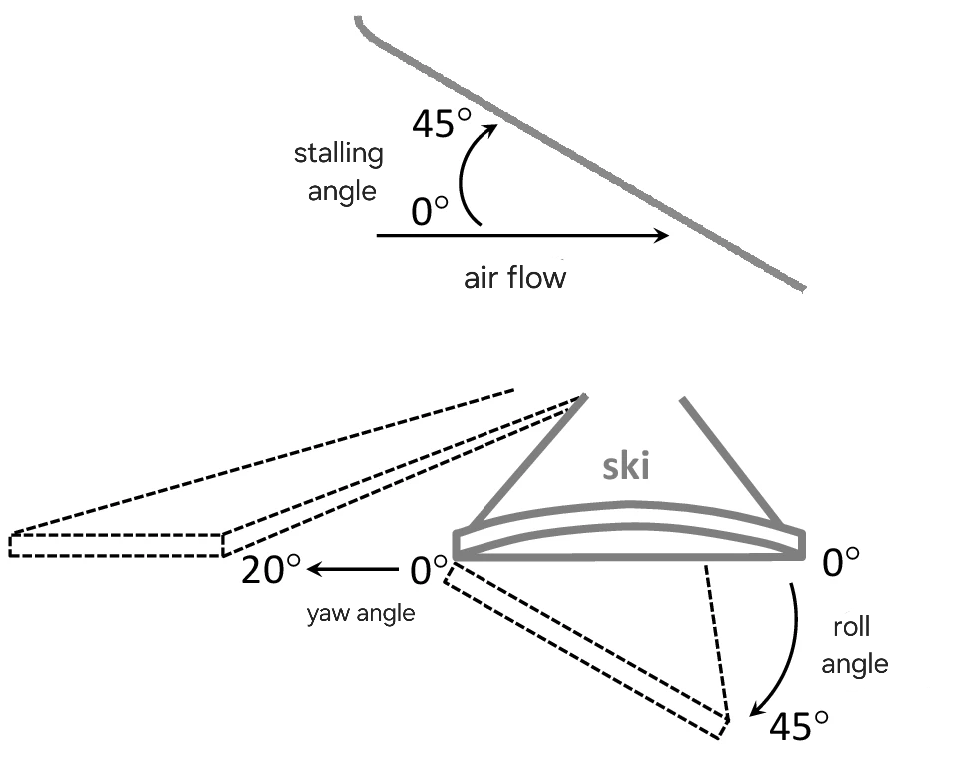
\includegraphics[width=0.5\linewidth]{koti.png}
      \caption{My first figure in beamer.}
      %\label{fig:question}
  \end{figure}
\end{frame}

\section{Methodology}

\subsection{Different approaches and error function}

\begin{frame}{Approach}
  \begin{enumerate}
    \item Step one
    \item Step two
    \item Step three
  \end{enumerate}
\end{frame}

\begin{frame}{Customized caption}
  \begin{figure}
  \centering
      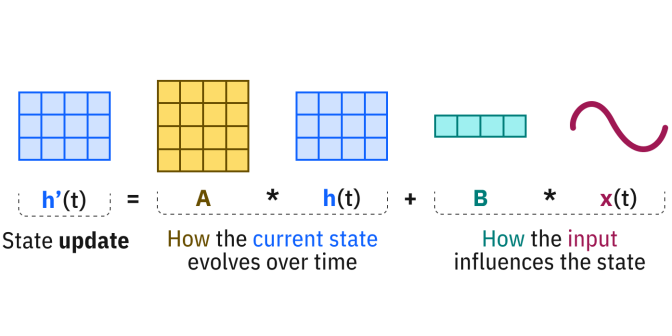
\includegraphics[width=0.5\textwidth]{SSM1.png}
      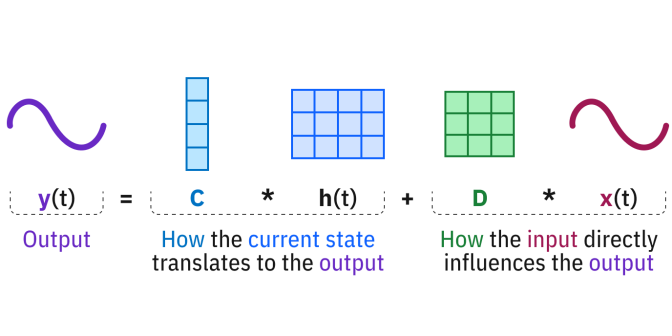
\includegraphics[width=0.5\textwidth]{SSM2.png}
      \caption{My first figure in beamer.}
      \label{fig:question}
  \end{figure}
\end{frame}

\subsection{Animation app}
\begin{frame}{App}
  \begin{itemize}
    \item Description of the app
    \item Key features
  \end{itemize}
\end{frame}

\section{Main Results}

\begin{frame}{Main Findings}
  \begin{block}{Key Result}
    Your important result goes here.
  \end{block}
\end{frame}

\begin{frame}{Customized caption}
\begin{figure}
\centering
    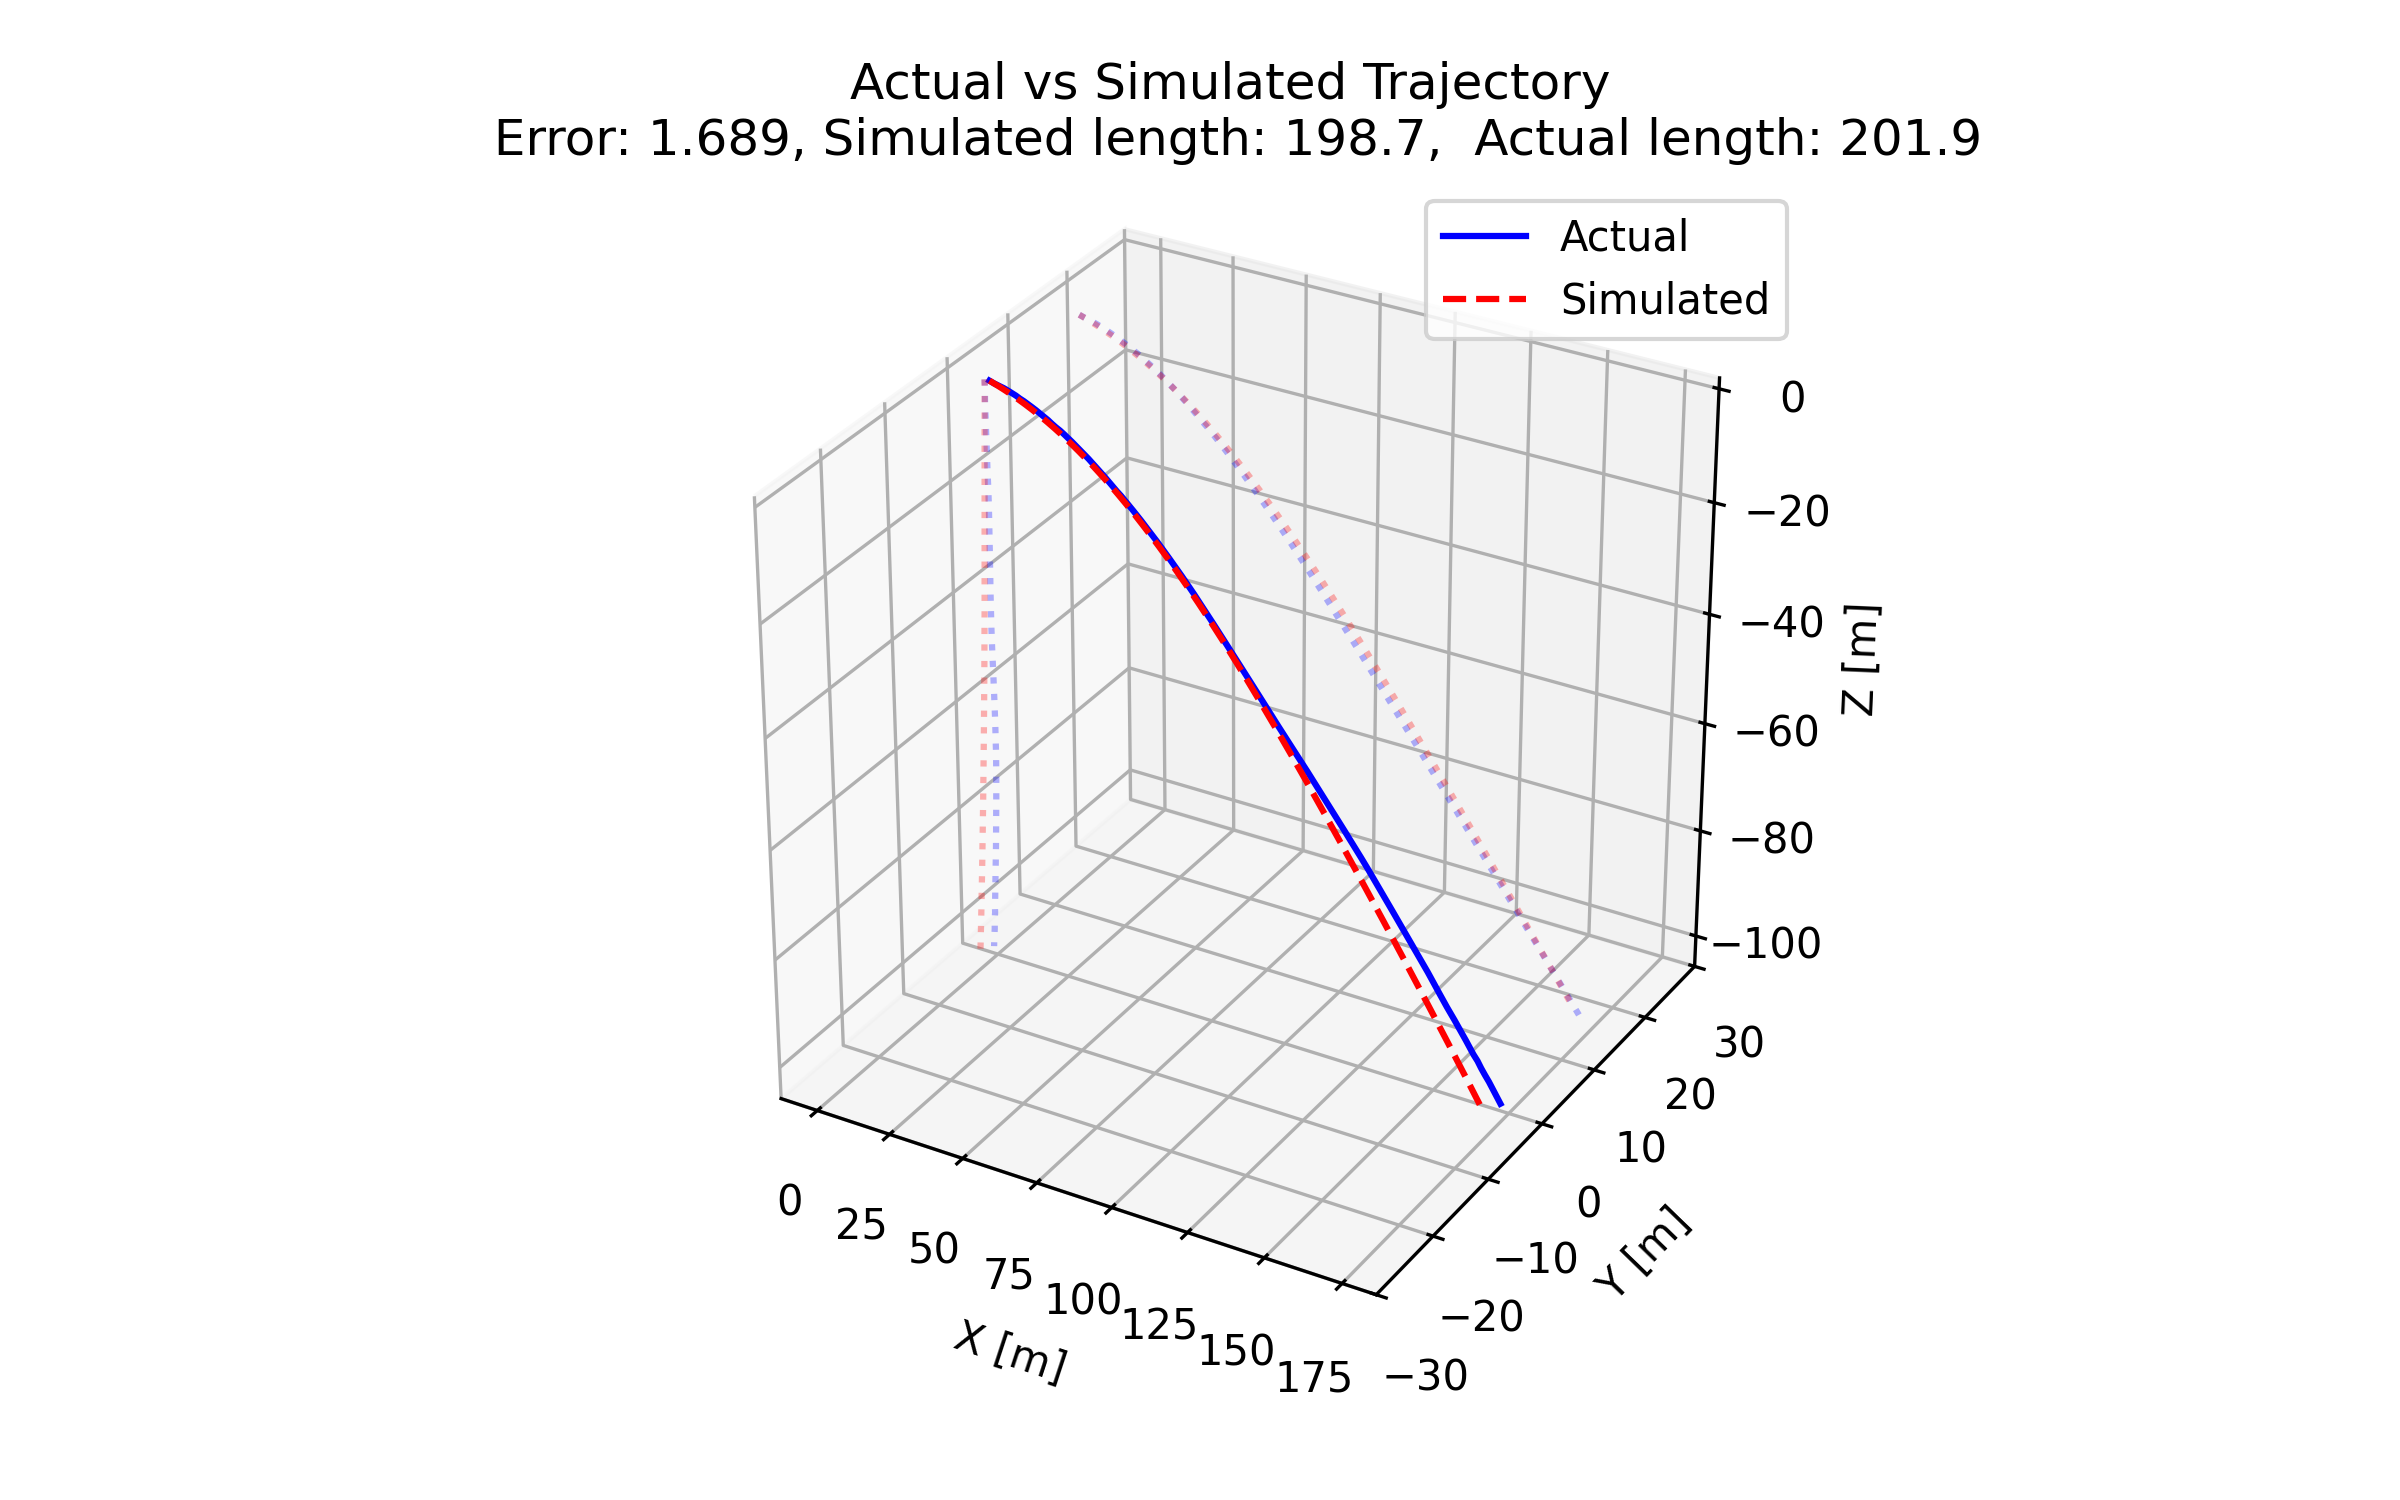
\includegraphics[width=0.5\textwidth]{flight_simulation167.png}
    \caption{My first figure in beamer.}
    \label{fig:question}
\end{figure}
\end{frame}

\section{Discussion and Conclusion}
\begin{frame}{Interpretation}
  \begin{itemize}
    \item Limitations
    \item Future work and potential improvements
    \item Short recap
  \end{itemize}
\end{frame}


% Thank you
\begin{frame}
  \centering
  \Huge Thank you!
\end{frame}

\end{document}
